\documentclass[ignorenonframetext]{beamer}
\usetheme{Hannover}
\usecolortheme{dove}
\usefonttheme{structurebold}
\usepackage{amssymb,amsmath}
\definecolor{links}{HTML}{2A1B81}
\hypersetup{colorlinks,linkcolor=,urlcolor=links}
\usepackage[T1]{fontenc}
\usepackage[utf8]{inputenc}
\usepackage{microtype}
\usepackage{longtable, booktabs}
\usepackage[english]{babel}
\usepackage{pgf, microtype, booktabs, times, etex}
\usepackage{tcolorbox}
\tcbuselibrary{minted,skins}

\newtcblisting{latexcode}{
	listing engine=minted,
	colback=bashcodebg,
	colframe=black!70,
	listing only,
	minted style=colorful,
	minted language=latex,
	minted options={linenos=true,texcl=true},
	left=1mm,
}
\definecolor{bashcodebg}{rgb}{0.85,0.85,0.85}
%\usemintedstyle{emacs}
\beamertemplatenavigationsymbolsempty

\title{\LaTeX{} for Economics and Business Administration}
\author{Thomas de Graaff}
\date{January 12, 2017}

\begin{document}
\frame{\titlepage}

\section{Introduction}\label{introduction}

\subsection{Why \& what}\label{introduction-1}

\begin{frame}{Why this workshop?}

\begin{itemize}
\item
  In the \emph{social sciences} few attention to what tools to use (and why)
  \newline
\item
  \LaTeX{} is very much used in the scientific world and \emph{works} brilliantly together with
  \begin{itemize}
  \item statistical packages, such as \texttt{Stata} and \texttt{R},
  \item markdown/HTML,
  \item reference managers.
  \newline
  \end{itemize}
  \item Why \emph{I} want to give this workshop
  \begin{itemize}
	  \item intrinsic interest
	  \item my goal: pre-conferences workshops / courses
  \end{itemize}
\end{itemize}
\end{frame}

\begin{frame}{What I want (and don't want) with this workshop}

\begin{itemize}
\item
  Give a general introduction of why some tools work together

  \begin{itemize}
  \item \LaTeX{}
  \item reference managers
  \item (statistical/structered) output
  \end{itemize}
\item
  Give an introduction to \LaTeX{}
  \begin{itemize}
	  \item First the basics + using references
	  \item Next workshop: some advanced stuff
  \end{itemize}
\item
  What \emph{I} do not want

  \begin{itemize}
  \item
    Tell you what applications to use (\textbf{you} need to decide and make a \textbf{well-informed} decision)
  \end{itemize}
\end{itemize}

\end{frame}

\texttt{\section{\LaTeX{}}\label{section}

\subsection{Introduction}\label{introduction-2}

\begin{frame}{Background}

\begin{itemize}
	\item \TeX{} has been devised by Donald E. Knuth in the 70's
	\newline
	\item \LaTeX{} is a set of macro's around TeX from the 80's
	\newline
	\item \LaTeX{} is a \emph{typesetting program}, not a \emph{Word processor}
  \begin{itemize}
  \item
    It is actually some code that needs to be compiled
  \item
    Code is typed in by an editor
    \newline
  \end{itemize}
\item
 So, 
  \begin{itemize}
  \item Huge differences between Word and \LaTeX{}
  \item for \LaTeX{} you need an editor:

    \begin{itemize}
    \item
      Specific editors: TexStudio, TexShop, RStudio
    \item
      General editors: Sublime, TextMate, Atom, Vim, Emacs
    \end{itemize}
  \end{itemize}
\end{itemize}

\end{frame}

\subsection{Why \LaTeX{}?}\label{why}

\begin{frame}{Disadvantages}

\begin{itemize}
\item
  Not WYSIWYG
\item
  You nead to learn (quite) some commands

  \begin{itemize}
  \item
    Learning curve, but
  \item
    hurray for
    \href{https://wch.github.io/latexsheet/latexsheet.pdf}{cheat sheets}
    and Google
  \end{itemize}
\item
  Difficult to cooperate with people from the \emph{dark side}
\item
  \emph{Basic} \LaTeX{} has \emph{difficulties} with incorporating new
  fonts (Hoefler, minion pro)

  \begin{itemize}
  \item
    XeTeX  \item
    For the purists: \LaTeX{} does it right
    \href{http://oestrem.com/thingstwice/2007/05/latex-vs-word-vs-writer/}{(\LaTeX{}
    vs Word)}
  \end{itemize}
  \item Difficult to create unstructured and ugly documents
\end{itemize}

\end{frame}

\begin{frame}{Advantages}

\begin{itemize}
\item Free (as in beer) and ubiquitous
\item WYSIWYM
\item Superior typography \& output  
\item Consistent lay-out throughout the whole document (including tables,
	  appendices, formulas, source code)
\item Internal references are a breeze (references, ToC, ToT)
\item Forced to structure documents
\item Macros, thus scriptable
\item Large community, thus a package for almost everything that you typeset on paper (books, articles, presentation, posters, exams, musicscores)
\item Many free \href{https://www.overleaf.com/latex/templates/}{\LaTeX~templates}
\end{itemize}

\end{frame}

\begin{frame}{\LaTeX{} versus Markdown}
	\begin{itemize}
		\item Markdown (all variants): lightweight markup language that can export to \texttt{.doc}, \texttt{.html}, and \texttt{.pdf}.
		\newline
		\item Much easier then \LaTeX{} but less flexible
		\newline
		\item Used by writers/blogs even for complete websites
		\newline
		\item But good interaction with \LaTeX{}; if not only for formula's
	\end{itemize}
\end{frame}

\subsection{Technicalities}\label{technicalities}

\begin{frame}[fragile]{How does \LaTeX{} work in practice?}

\begin{itemize}
\item
  You edit a \texttt{.tex} file without thinking about how it looks

  \begin{itemize}
  \item
    distraction free writing (yeah right)
    \newline
  \end{itemize}
\item
  You then compile it

  \begin{itemize}
  \item
    \LaTeX{} is unforgiving: if there is an error, usually it does not
    compile
  \item
    Typically, errors are missing brackets or parentheses.\newline
  \end{itemize}
\item
  Typically, source \texttt{.tex} file is compiled into \texttt{.pdf}
\end{itemize}

\end{frame}

\begin{frame}{A process diagram}

\begin{figure}[htbp]
\centering
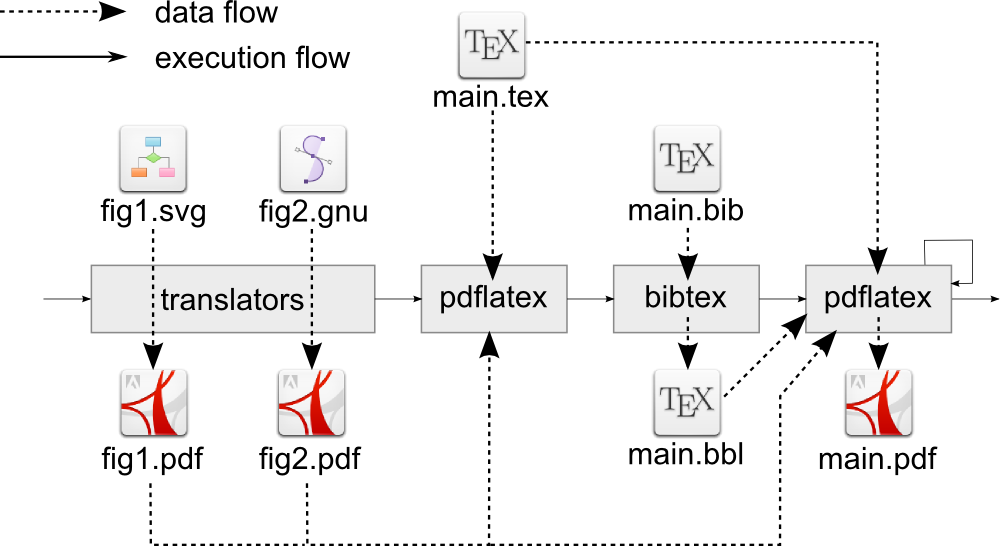
\includegraphics[width=\textwidth]{fig/process.png}
\caption{Process diagram}
\end{figure}

\end{frame}

\begin{frame}[fragile]{Code, documentation and output}

\begin{enumerate}
\def\labelenumi{\arabic{enumi}.}
\item
  Synonyms
\item
  All based on \texttt{.txt} files
\item
  Encompasses almost anything

  \begin{itemize}
  \item
    data itself (\texttt{.csv}, \texttt{.txt})
  \item
    set of commands for data cleaning and statistical analysis
    (\texttt{.do}, \texttt{.R})
  \item
    database with references (\texttt{.bib})
  \item
    text for articles, presentations or websites (\texttt{.tex},
    \texttt{.html})
  \end{itemize}
\item
  Only output is displayed/interpreted differently (e.g., in a browser
  or pdf viewer)
\end{enumerate}

\end{frame}

\subsection{Folder structure and file
names}\label{folder-structure-and-file-names}

\begin{frame}{Folder structure of your new project (theses, paper, assignment \& research)}

\begin{itemize}
\item
  Think \emph{a priori} about project set-up

  \begin{itemize}
  \item
    Seperate analysis, data and output files
  \end{itemize}
\item
  Be careful with source data!

  \begin{itemize}
  \item
    Seperate source and derived data files
  \item
    Typically

    \begin{itemize}
    \item
      you get/collect data
    \item
      transform data
    \item
      analyse data
    \end{itemize}
  \item
    Keep track of all these stages!
  \end{itemize}
\end{itemize}
\end{frame}


\section{TeXstudio}

\subsection{How to work with TeXstudio}

\begin{frame}{TeXstudio: A quick tour}
	\begin{itemize}
		\item Preferences
		\newline
		\item Keyboard shortcuts
		\newline
		\item LaTeX dropdown menu
	\end{itemize}
\end{frame}

\section{Exercises}

\subsection{Baby-steps}

\begin{frame}{First: organize!}
	\begin{enumerate}
		\item Create a specific workshop folder somewhere where you can find it.
		\newline
		\item Think about versioning system and a back-up system
		\newline
		\item E.g.: use dropbox and/or Time Machine 
	\end{enumerate}
\end{frame}

\begin{frame}[fragile]{Exercise 1: Open from template and fill in!}
\small
\begin{latexcode}
\documentclass[]{article}
%opening
\title{}
\author{}

\begin{document}
	
\maketitle

\begin{abstract}
	
\end{abstract}

\section{}
	
\end{document}
\end{latexcode}
\end{frame}

\begin{frame}{OK; and now what?}
	\begin{enumerate}
		\item Save your file in your folder (give it an appropriate name)
		\newline
		\item Press \texttt{F1} (or \texttt{F5})
		\newline
		\item The editor now sends \LaTeX{} the message that it should \textit{compile} your file
		\newline
		\item \LaTeX{} creates many new files
	\end{enumerate}
\end{frame}

\subsection{Paper structure}

\begin{frame}[fragile]{Exercise 2: Create a paper structure}
	\small
	\begin{latexcode}
\section{}
\subsection{}
\subsubsection{}
	\end{latexcode}
Note that the following are used for books
\small
\begin{latexcode}
\part{}
\chapter{}
\end{latexcode}
And for bigger projects:
\begin{latexcode}
\include{}
\input{}
\end{latexcode}
\end{frame}

\begin{frame}[fragile]{Intermezzo: preamble}
Part before \texttt{\textbackslash begin\{document\}} is called preamble\\
A set of \texttt{[]} indicates options for the given command
\begin{latexcode}
\documentclass[]{article}

% This is where packages are loaded 
% and specific commands are given that 
% determine how the lay-out and desing
% of your document will look like 
% including: references, tables, 
% paragraphs, headers, etc.
	
\begin{document}
\end{latexcode}	
\end{frame}

\begin{frame}[fragile]{Intermezzo: white spaces and special characters}
An empty line starts a new paragraph and consecutive white spaces are treated as one
\begin{latexcode}
One paragraph

Second     paragraph (just one white space)
\end{latexcode}	

The following characters are reserved \# \$ \% \^{} \& \_ \{ \} \~{} \textbackslash{} and should be used as follows
\begin{latexcode}
\# \$ \% \^ \& \_ \{ \} \~ 
\textbackslash
\end{latexcode}	
So, with a backslash before except for the backslash (does this make sense?)
\end{frame}

\begin{frame}[fragile]{Exercise 3: Create a table of contents}
More complex text structures are relatively easy, just insert (after \texttt{\textbackslash begin\{document\}})
\begin{latexcode}
\tableofcontents
\listoffigures
\listoftables
\end{latexcode}
\end{frame}

\begin{frame}[fragile]{Lists}
\begin{itemize}
	\item Itemization
\begin{latexcode}
\begin{itemize}
	\item blue
	\item red
\end{itemize}
\end{latexcode}	
	\item Enumeration
\begin{latexcode}
\begin{enumerate}
	\item first item
	\item second item
\end{enumerate}
\end{latexcode}	
\end{itemize}
\end{frame}

\begin{frame}[fragile]{Exercise 4: Lists}
	Create the following mode choice list in your \texttt{.tex} document\\
	\\
	\begin{enumerate}
		\item Cycling
		\item Walking
		\item Driving
		\item Public transport
		\begin{itemize}
			\item Bus
			\item Tram
			\item Metro
			\item Train
		\end{itemize} 
	\end{enumerate}
\end{frame}

\begin{frame}[fragile]{Further text control}
\begin{itemize}
\item Bold
\begin{latexcode}
\textbf{bold}
\end{latexcode}		
\item Emphasize
\begin{latexcode}
\textit{italics} or \emph{emphasized}
\end{latexcode}		
\end{itemize}
\end{frame}

\subsection{Formula's} 

\begin{frame}[fragile]{Formula's}
Inline math \texttt{\$ \$}; displayed math \texttt{\$\$ \$\$}; for example:
\begin{latexcode}
$x^2$
$x_2$
$\sqrt{x}$
$$Y = K^\alpha L^{1-\alpha}$$
$$\sum_{i=1}^I$$
$$\frac{\partial x}{\partial y}$$
\begin{equation}
	E = mc^2
\end{equation}
\end{latexcode}
\end{frame}

\begin{frame}{Exercise 5: Create these formula's}
	\begin{enumerate} 
		\item Regression formula:
		\[ y_i = \alpha + \beta x_i + \epsilon_i \]
		\item The mean
		$$\bar{x} = \frac{1}{N}\sum_{i=1}^N x_i$$
		\item Optimal economic order quantity:
		$$Q^\ast = \sqrt{ \frac{2DK}{h}} $$
	\end{enumerate}
\end{frame}

\subsection{Figures}

\begin{frame}[fragile]{Figures}
	Figures/graphs and tables in a floating environment\\
\begin{latexcode}
\begin{figure}[h!]}
\center
	
\includegraphics{ligatures_latex}
	\caption{A figures about ligatures}
	\label{fig:ligatures}
\end{figure}
\end{latexcode}
Figures can be \texttt{.pdf}, \texttt{.jpg}, \texttt{.png} and a whole lot of other types (but not bitmaps!)
\end{frame}

\subsection{Tables}

\begin{frame}[fragile]{Tables}
\begin{latexcode}
\begin{table}[t!]
	\caption{This is the caption}
	\begin{tabular}{|l|c|r|}
		\hline
		first & row & data \\
		second & row & data \\
		\hline
	\end{tabular}
	\label{tab:example}
\end{table}
\end{latexcode}
\end{frame}

\subsection{Referencing}

\begin{frame}[fragile]{Referencing}
Internal references are a breeze
\begin{latexcode}
\label{}	% Label something
\ref{}	% Refer to that
\footnote{}	% Add footnote
\thanks{}	% For in title
\end{latexcode}
\end{frame}

\begin{frame}[fragile]{Exercise 6: Create a table}
Create the following table 

\begin{table}[!th]
	\center
	\caption{Average grades}
	\begin{tabular}{lrr}
		\hline
		First name  & Surname & Grade \\
		\hline
		Sherlock & Holmes & 7.9 \\
		John H. & Watson & 8.1 \\
		\hline
		\\
		\\
	\end{tabular}
	\label{tab:grades}
\end{table}

And refer to it in text as such: 
\begin{quote}
	Table \ref{tab:grades} gives the average grades for the course \textbf{Solving Crimes}.
\end{quote}
\end{frame}

\begin{frame}[fragile]{BibTeX}
Literature references (at the end)
\begin{latexcode}
\cite{} % cite something
% Now tell LaTeX where to find references	
\bibliography{references.bib}
% and which citation style to use
\bibliographystyle{apalike}
\end{latexcode}
Later, we dive into how to make this look good
\end{frame}

\begin{frame}{Exercise 7: References}
	\begin{enumerate}
		\item Search on Google Scholar for three references from Erik Verhoef and/or Wout Dullaert
		\newline
		\item Put those in a \texttt{.bib} file in the \textbf{same} directory as your \texttt{.tex} file
		\newline
		\item Refer to those in your \texttt{.tex} file
		\newline
		\item Create the reference list
	\end{enumerate}
\end{frame}

\section{Conclusion}

\subsection{Next time}

\begin{frame}{Next workshop}
	\begin{itemize}
		\item Use of packages
		\newline
		\item Making things look better!
		\newline
		\item Graphs
		\newline
		\item Better tables with \texttt{Stata} and \texttt{R} output
		\newline
		\item Slides
	\end{itemize}
\end{frame}

\end{document}

%%% Local Variables:
%%% mode: latex
%%% TeX-master: t
%%% End:
